\section{Key Insights}

\begin{figure}[t!]
    \centering
    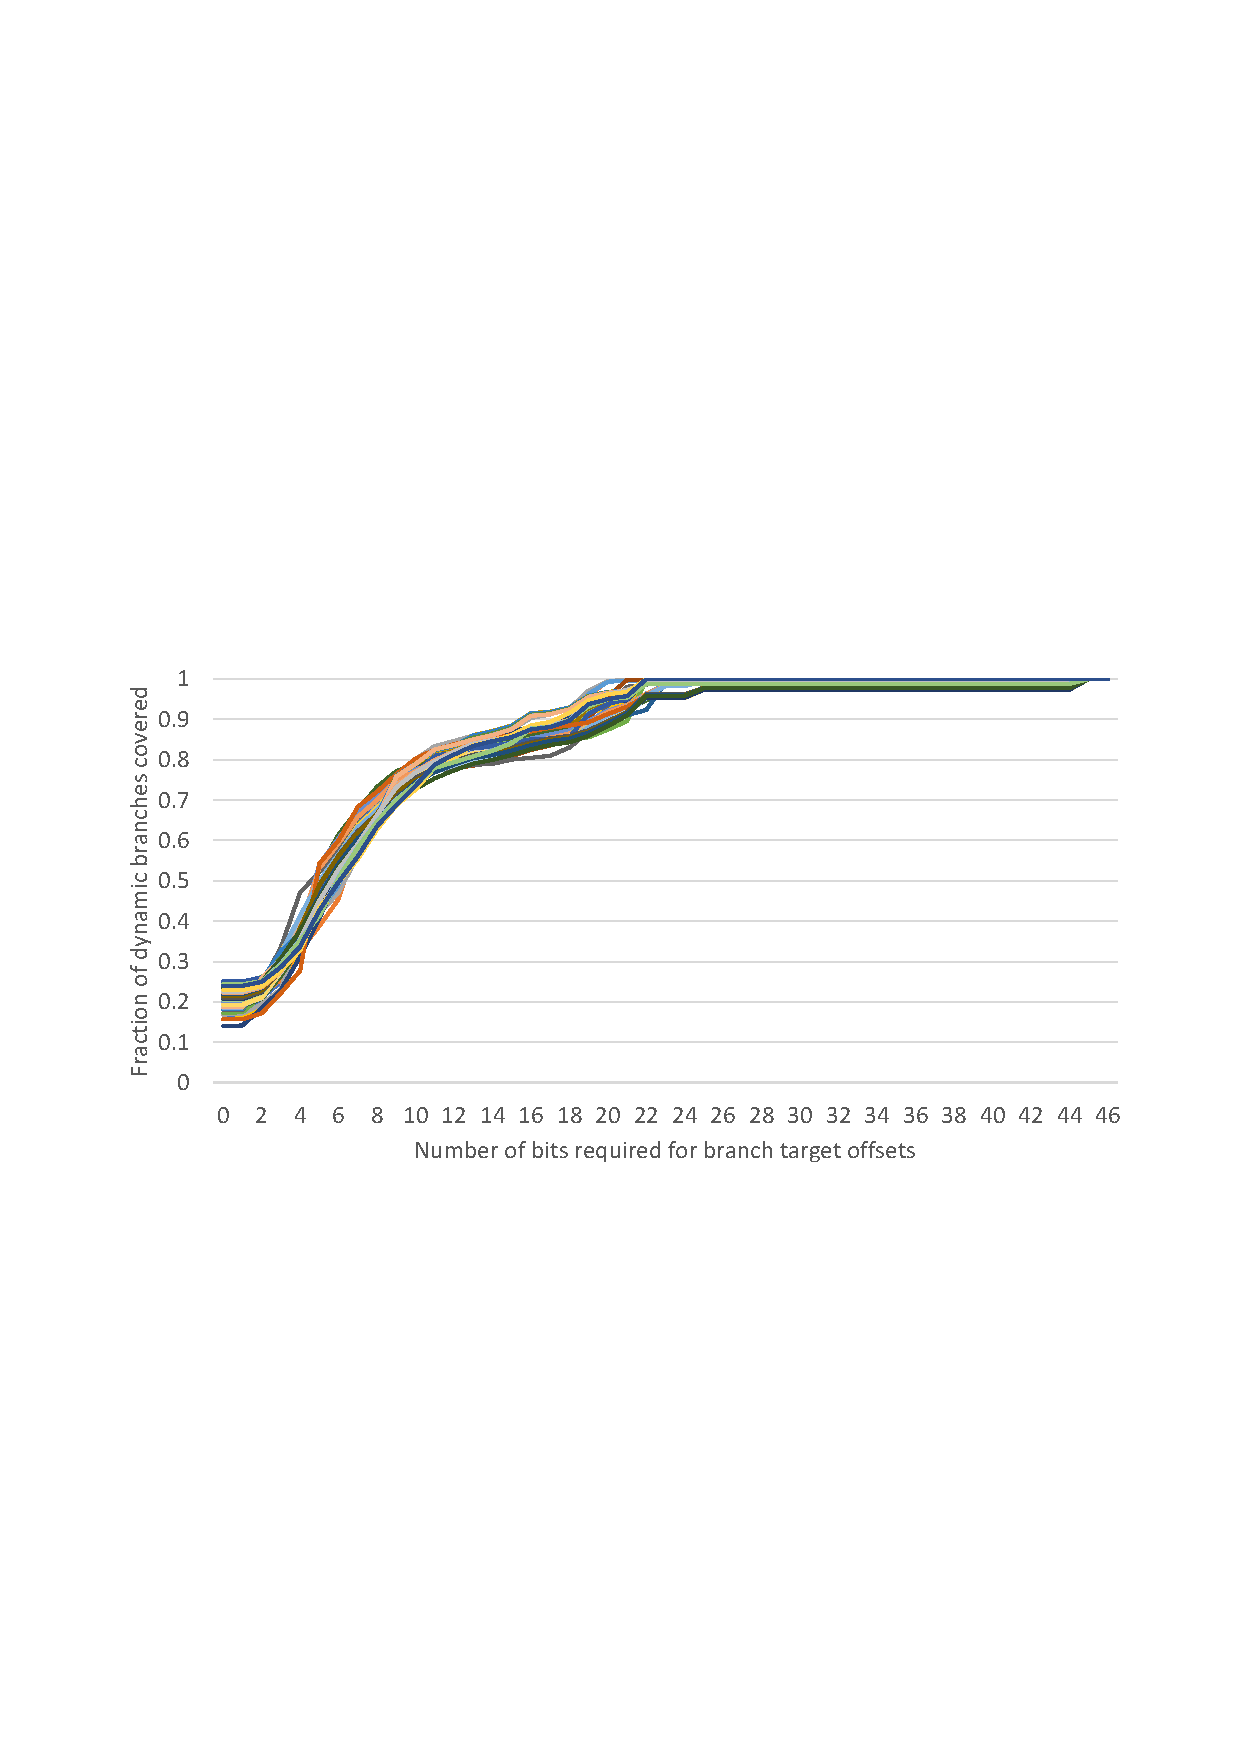
\includegraphics[width=\columnwidth, trim=60 280 50 320, clip]{figures/offset_distribution.pdf}
    \vspace{-0.25in}
    \caption{Distribution of branch target offsets.}
    \vspace{-0.25in}
    \label{pact:fig:offsets}
\end{figure}

We analyze conventional and state-of-the-art BTB organizations and observe that the branch targets are the single largest contributor to BTB storage cost. Further, we analyze the number of bits required for branch target \emph{offsets} to assess if storing the offsets, instead of the full or compressed targets, can reduce BTB storage requirements. 

\Cref{pact:fig:offsets} plots the distribution of branch target offsets in the branch working sets of our workloads. The data includes both conditional and unconditional branches; hence, it comprehensively covers the full branch working set. The X-axis shows the number of bits required to store offsets, while the Y-axis plots the fraction of dynamic branches covered.

As the figure shows, short offsets dominate the distribution with 54\% of branches requiring only six bits or fewer for their offsets. A further 22\% of branches only require between 7 and 10-bits to represent their offsets. The reason why such a high fraction of offsets is short is that conditional branches dominate the dynamic branch working set, and they tend to have short offsets~\cite{boomerang}. This is because conditional branches generally guide the control flow only inside a function; meanwhile, software engineering principles favor small functions, thus restricting conditional branch target offsets to short distances. Furthermore, return instructions get their target from the return address stack (RAS), thus they do not need to store any target bits in BTBs. Therefore, for the purpose of this analysis, we assume 0-bit offsets for return instructions.

Perhaps surprisingly, \Cref{pact:fig:offsets} also shows that very few branches require a large number of bits for their offset. Indeed, a meagre 1\% of branches requires more than 25 bits for their offsets. The sum of these results indicates that reserving space for the full 46-bit target address results in an appalling under-utilization of BTB storage, since 99\% of branches need at most half the number of bits needed to represent the full target address if offsets are used instead.

We gain two key insights from this analysis:

\begin{description}
\item[Key Insight 1] The targets of most branches lie relatively close in the virtual address space to the branch itself. As a result, storing the {\em distance} to the target, in the form of an offset from the branch instruction can provide drastic storage savings. 

\item[Key Insight 2] The target offset sizes are unevenly distributed with 0-6 bits, 7-10 bits, and 11-25 bits required to encode the offsets of 54\%, 22\% and 23\% of branches respectively. Therefore, a single size offset field cannot provide storage optimal solution.
\end{description}
